\documentclass{book}
\usepackage{html}
\usepackage{fancyheadings}
\usepackage{graphicx}

\newcommand{\gnutls}{{\emph{GNUTLS}} }
\newcommand{\tls}{{\emph{TLS}} }
\newcommand{\ssl}{{\emph{SSL}} }
\newcommand{\HRule}{\rule{\linewidth}{0.4mm}}


\begin{document}

\pagenumbering{roman}

\thispagestyle{empty}

\setlength{\parindent}{0mm}

\setlength{\parskip}{0mm}

 {\Huge GNUTLS\\[.1mm]}
 \HRule
 \begin{flushright}
  a Transport Layer Security Library
 \end{flushright}

 \vspace*{\stretch{3}}

 {\Large By Nikos Mavroyanopoulos and Fabio Fiorina\\[.1mm]}
 \HRule
 
\newpage

\vspace*{\stretch{2}}

\begin{center}
\par
Permission is granted to copy, distribute and/or modify this
document under the terms of the GNU Free Documentation License,
Version 1.1 or any later version published by the Free Software
Foundation; with no Invariant Sections, no Front-Cover Texts and
no Back-Cover Texts.  A copy of the license is included in the
chapter entitled "GNU Free Documentation License".
\end{center}



\tableofcontents
\newpage
\pagenumbering{arabic}
\pagestyle{fancy}

\chapter{The Library}
\section{Introduction}
\par
\gnutls{} is a portable library which implements the \tlsI{} and 
\sslIII{} protocols.
\tls{} stands for 'Transport Layer Security' and is the sucessor of \ssl{}, 
the Secure Sockets Layer protocol designed by Netscape. 

\tlsI{}\footnote{described in {\it RFC 2246}} is an Internet protocol,
defined by {IETF}\footnote{IETF or Internet Engineering Task Force 
is a large open international community of network
designers, operators, vendors, and researchers concerned with the evolution of 
the Internet architecture and the smooth operation of the Internet. It is open to any interested individual.}, 
that provides confidentiality, and authentication layers over any
transport layer.

\par
\gnutls{} implements the above
protocols in a reentrant way. This allows multiple threads of
execution, without the need for Critical Sections and locks. See
\htmladdnormallink{http://www.gnutls.org/}{http://www.gnutls.org/}
and \htmladdnormallink{http://www.gnu.org/software/gnutls/}{http://www.gnu.org/software/gnutls/} 
for updated versions of the \gnutls{} software and this document.

\par
Currently \gnutls{} implements:
\begin{itemize}
 \item the \tlsI{} and \sslIII{} protocols, without any weak algorithms\footnote{
There are ciphersuites in \tlsI{} that are considered weak. These
ciphersuites are deliberately weak in order to be able to export encryption
software from some countries.}
 \item {\bf X.509} Public Key Infrastructure.
 \item {\bf OpenPGP} Public Key Infrastructure.
 \item {\bf SRP} for \tls{} authentication.
 \item \tls{} {\bf Extension mechanism}.
\end{itemize}

\newpage
\section{TLS layers}

\tlsI{} is a layered protocol, and consists of the Record Protocol,
the Handshake Protocol and the Alert Protocol. The Record Protocol
is to serve all other protocols and is above the transport layer.
The Record protocol offers symmetric encryption, and data authenticity.
In \gnutls{} the record protocol is accessed using the 
\hyperref{gnutls\_record\_read()}{gnutls\_record\_read() (see Section }{)}{gnutls_record_read} and
\hyperref{gnutls\_record\_write()}{gnutls\_record\_write() (see Section }{)}{gnutls_record_write}
functions.

\par
The Alert protocol offers some signaling to the other protocols. It can
help informing the peer for the cause of failures and other error
conditions.
\hyperref{gnutls\_alert\_send()}{gnutls\_alert\_send() (see Section }{)}{gnutls_alert_send} and
\hyperref{gnutls\_alert\_send\_appropriate()}{gnutls\_alert\_send\_appropriate() (see Section }{)}{gnutls_alert_send_appropriate} 
functions.

\par 
The Handshake protocol is responsible for the initial key exchange,
and authentication. See \hyperref{figure}{figure }{}{fig:cert} for the
protocol layering in TLS. The handshake protocol in \gnutls{} is accessed
with the 
\hyperref{gnutls\_handshake()}{gnutls\_handshake() (see Section }{)}{gnutls_handshake} function.

\begin{figure}[hbtp]
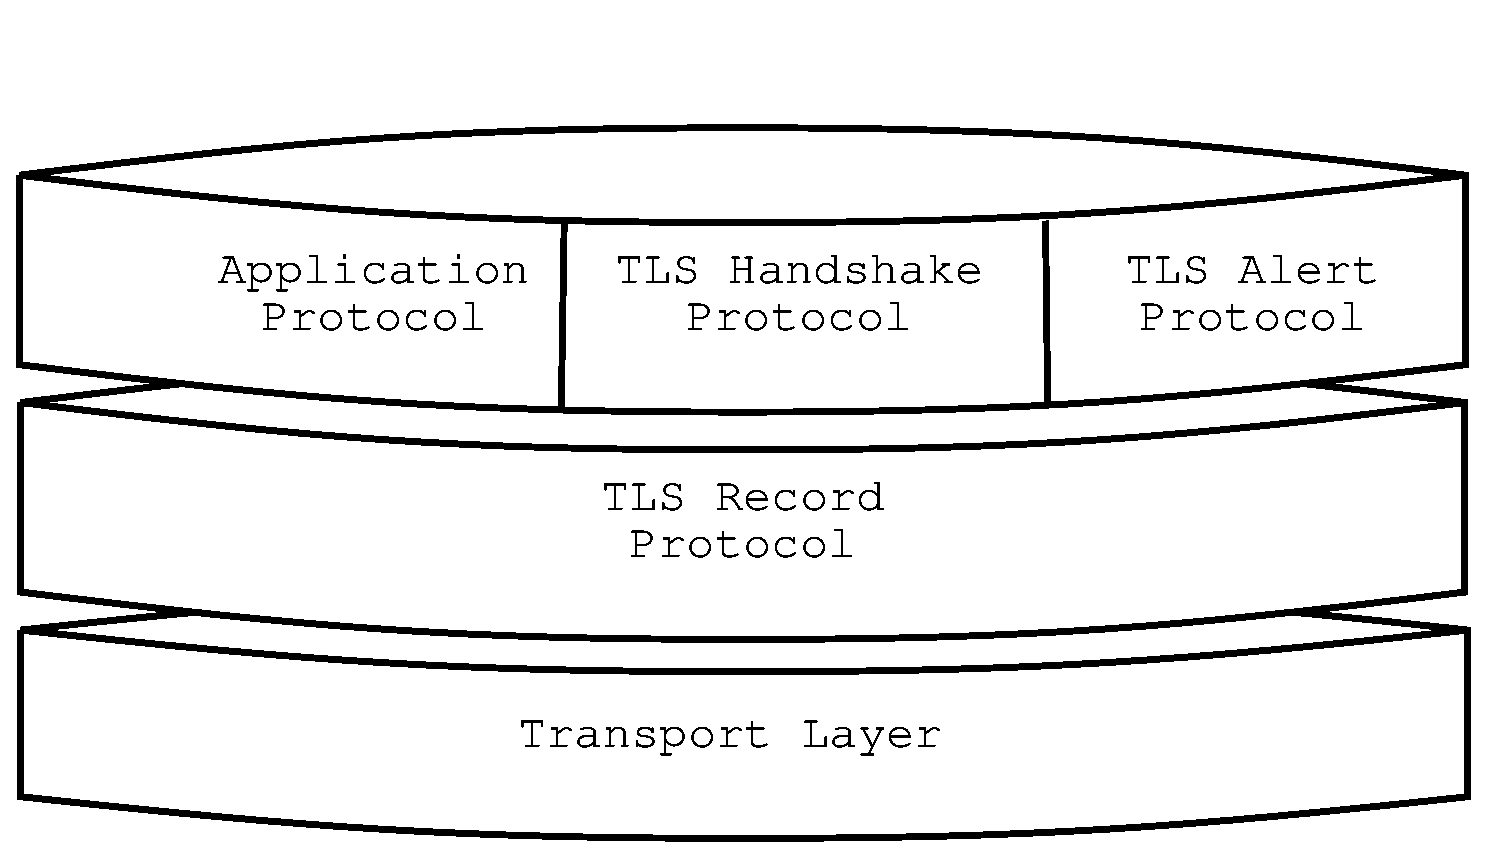
\includegraphics{layers}
\label{fig:layers}

\end{figure}


\addvspace{1.5cm}



\subsection*{TLS cipher suites}
\par 
The Handshake Protocol of \tlsI{} negotiates cipher suites 
of the form \\
{\bf TLS\_DHE\_RSA\_WITH\_3DES\_CBC\_SHA}.
The usual cipher suites contain these parameters:
\begin{itemize}
\item The key exchange algorithm ---DHE\_RSA in the example.
\item The Symmetric encryption algorithm and mode ---3DES\_CBC in this
example.
\item The MAC\footnote{MAC stands for Message Authentication Code. It can
be described as a keyed hash algorithm. See RFC2104.} algorithm used for authentication.
MAC\_SHA is used in the above example.
\end{itemize}

The cipher suite negotiated in the handshake protocol will affect
the Record Protocol, by enabling encryption and data authentication.
Note that you should not over rely on \tls{} to negotiate the strongest 
available cipher suite. Do not enable ciphers and algorithms that you consider weak.
\par
The priority functions, dicussed above, allow the application layer to enable
and set priorities on the individual ciphers. It may imply that all combinations of ciphersuites
are allowed, but this is not true. For several reasons, not discussed here, some combinations 
were not defined in the \tls{} protocol. The supported ciphersuites are shown
in appendix \ref{ap:ciphersuites} on page \pageref{ap:ciphersuites}.

\addvspace{1.5cm}


\section{Authentication methods}
\par
The following authentication schemas are supported in \gnutls:
\begin{enumerate}
 \item X509 Public Key Infrastructure
 \item Anonymous authentication
 \item SRP authentication
\end{enumerate}

\subsection{Authentication using X.509 certificates}
If using this kind of authentication then the key exchange methods
shown in \hyperref{figure}{figure }{}{fig:x509} are
available to use. Authentication in this method is performed using signed
certificates by a trusted Certificate Authority (CA). Note that \gnutls is
not a generic purpose X.509 toolkit\footnote{Aegypten is such a toolkit. See http://www.gnupg.org/aegypten/}. 
It does only include the required,
in order to use the TLS ciphersuites which require X.509 certificates.

\begin{figure}[hbtp]
\begin{tabular}{|l|p{9cm}|}
\hline
X509PKI\_RSA & The RSA algorithm is used to encrypt a key and send it to the peer.
The certificate must allow the key to be used for encryption.
\\
\hline
X509PKI\_DHE\_RSA & The RSA algorithm is used to sign Ephemeral Diffie Hellman
parameters which are send to the peer. The key in the certificate must allow
the key to be used for signing 
\\
\hline
X509PKI\_DHE\_DSS & The DSS\footnote{DSS stands for Digital Signature Standard} algorithm is used to sign Ephemeral Diffie Hellman
parameters which are send to the peer. Currently \gnutls does not support this ciphersuite.
\\
\hline
\end{tabular}

\caption{Supported X.509 key exchange algorithms}
\label{fig:x509}

\end{figure}

\subsection{Anonymous authentication}
The anonymous key exchanges perform encryption but there is no indication of the 
identity of the peer. This kind of authentication is vulnerable to man in the middle attack, 
but this protocol can be used even if there is no prior communication or common trusted
parties with the peer. Unless really required, do not use anonymous authentication.
Available key exchange methods are shown in \hyperref{figure}{figure }{}{fig:anon}.

\begin{figure}[hbtp]
\begin{tabular}{|l|p{9cm}|}

\hline
ANON\_DH & This algorithm exchanges Diffie Hellman parameters. 
\\
\hline
\end{tabular}

\caption{Supported anonymous key exchange algorithms}
\label{fig:anon}

\end{figure}

\subsection{Authentication using SRP}
Authentication using the SRP\footnote{SRP stands for Secure Password Protocol and 
is described in RFC2945. The SRP key exchange is not a part of the \tlsI protocol}
can be described as password authentication, since the two peers are identified by the knowledge 
of a password. This protocol also offers protection against off-line attacks (password file stealing
etc.). 
Available key exchange methods are shown in \hyperref{figure}{figure }{}{fig:srp}.

\begin{figure}[hbtp]
\begin{tabular}{|l|p{9cm}|}

\hline
SRP & Authentication using the SRP protocol. 
\\
\hline
\end{tabular}

\caption{Supported SRP key exchange algorithms}
\label{fig:srp}

\end{figure}


\subsection{Encryption algorithms used in the record layer}
\index{Symmetric encryption algorithms}
Confidentiality in the record layer is achieved by using symmetric block 
encryption algorithms like {\bf 3DES}, {\bf AES\footnote{AES or Advanced 
Encryption Standard is actually the RIJNDAEL algorithm. This is the
algorithm that replaced DES.}}, or
stream algorithms like {\bf ARCFOUR\_128\footnote{ARCFOUR\_128 is a compatible
algorithm with RSA's RC4 algorithm, which is considered to be a trade secret.}} See \hyperref{fig:ciphers}{figure }{}{fig:ciphers} for a complete list. 
Ciphers are encryption algorithms that use a single (secret) key
to encrypt and decrypt data. Block algorithms in TLS also provide protection
against statistical analysis of the data. \gnutls{} makes use of this property
thus, if you're using the \tlsI{} protocol, a random number of blocks will be
appended to the data. This will prevent eavesdroppers from guessing the 
actual data size.

\begin{figure}[hbtp]
\begin{tabular}{|l|p{9cm}|}

\hline
3DES\_CBC & 3DES\_CBC is the DES block cipher algorithm used with triple
encryption (EDE). Has 64 bits block size and is used in CBC mode.
\\
\hline
ARCFOUR\_128 & ARCFOUR is a fast stream cipher.
\\
\hline
ARCFOUR\_40 & This is the ARCFOUR cipher that is fed with a 40 bit key,
which is considered weak.
\\
\hline
AES\_CBC & AES or RIJNDAEL is the block cipher algorithm that replaces 
the old DES algorithm. Has
128 bits block size and is used in CBC mode. This is not officially
supported in TLS.
\\
\hline
\end{tabular}
\caption{Supported cipher algorithms}
\label{fig:ciphers}
\end{figure}



\addvspace{1.5cm}

\begin{figure}[hbtp]
\begin{tabular}{|l|p{9cm}|}

\hline
MAC\_MD5 & MD5 is a cryptographic hash algorithm designed by Ron Rivest. Outputs 128 bits of data.
\\
\hline
MAC\_SHA & SHA is a cryptographic hash algorithm designed by NSA. Outputs 160 bits of data.
\\
\hline
MAC\_RMD160 & RIPEMD is a cryptographic hash algorithm developed in the framework
of the EU project RIPE. Outputs 160 bits of data.
\\
\hline
\end{tabular}
\caption{Supported MAC algorithms}
\index{MAC algorithms}
\label{fig:mac}
\end{figure}



\section{Resuming Sessions}
\par
The 
\hyperref{gnutls\_handshake()}{gnutls\_handshake() (see Section }{ for more information)}{gnutls_handshake}
 function, is expensive since a lot of calculations are performed. In order to support many fast connections to
the same server a client may use session resuming. {\bf Session resuming} is a
feature of the {\bf TLS} protocol which allows a client to connect to a server,
after a successful handshake, without the expensive calculations (by using the previously
established keys). \gnutls supports this feature, and the
example \hyperref{resume client}{resume client (see Section }{ for more
information)}{resume-example} illustrates a typical use of it (This is a modification of the simple client example).
Servers only need to use the
\hyperref{gnutls\_set\_db\_name()}{gnutls\_set\_db\_name() (see Section }{ for more
information)}{gnutls_set_db_name} function if they want to use the gdbm
backend to store sessions. 
\par
Keep in mind that sessions are expired after some time (for security reasons), thus
it may be normal for a server not to resume a session even if you requested that.
Also note that you must enable (using the priority functions), at least the
algorithms used in the last session.

\subsection{Resuming internals}
The resuming capability (mostly in the server side) is one of the problems of a thread-safe TLS
implementations. The problem is that all threads must share information in
order to be able to resume sessions. The gnutls approach is, in case of a
client, to leave all the burden of resuming to the client (ie. copy and keep the
nesessary parameters etc.).
\par
The server side is different\footnote{Future versions of gnutls may be
different}. 
Here the server only specifies a DB file (using 
\hyperref{gnutls\_set\_db\_name()}{gnutls\_set\_db\_name() (see Section }{ for more
information)}{gnutls_set_db_name}
) to be used. This DB file is used to store the sessions' required parameters for
resuming (and this means that this file contains very sensitive information,
such as encryption keys). In a multi-threaded application every thread can
read from the DB file and access all previously established sessions, but
only one thread can write at a time. The current behaviour of gnutls is
not to block and wait for the DB to be ready for writing, but continue the
process normally (and do not save the parameters).  
\par
 After version {\emph 0.2.10} \gnutls provides callback functions such as:
\hyperref{gnutls\_set\_db\_remove\_function()}{gnutls\_set\_db\_remove\_function() (see Section }{ for more
information)}{gnutls_set_db_remove_function},
\hyperref{gnutls\_set\_db\_store\_function()}{gnutls\_set\_db\_store\_function() (see Section }{ for more
information)}{gnutls_set_db_store_function},
\hyperref{gnutls\_set\_db\_retrieve\_function()}{gnutls\_set\_db\_retrieve\_function() (see Section }{ for more
information)}{gnutls_set_db_retrieve_function} and
\hyperref{gnutls\_set\_db\_ptr()}{gnutls\_set\_db\_ptr() (see Section }{ for more
information)}{gnutls_set_db_ptr}.
These callback functions are required in order to use a session
storage method, other than the default gdbm backend. 
\par
If an alternative backend is in use, it might be usefull to be able to check
for expired sessions in order to remove them, and save space (in the way 
\hyperref{gnutls\_clean\_db()}{gnutls\_clean\_db() (see Section }{ for more
information)}{gnutls_clean_db}.
) does for the gdbm backend. \gnutls provides the function
\hyperref{gnutls\_check\_db\_entry()}{gnutls\_check\_db\_entry() (see Section }{ for more
information)}{gnutls_check_db_entry}, which takes as input session data, and
returns a negative value if the data are to be removed.



\section{Transport Layer}
\par
\gnutls can be used above any transport layer. To do this you will only 
need to set up the 
\hyperref{gnutls\_transport\_set\_push\_function()}{gnutls\_transport\_set\_push\_function() (see Section }{
for more information)}{gnutls_transport_set_push_function} and
\hyperref{gnutls\_transport\_set\_pull\_function()}{gnutls\_transport\_set\_pull\_function() (see Section }{
for more information)}{gnutls_transport_set_pull_function}
functions. These functions will then be used by gnutls in order to send and receive data.
The functions specified should return -1 on error and should set errno appropriately.
\gnutls supports EINTR and EAGAIN errno values. These values are
usually used in non blocking IO and interrupted system calls.
The corresponding values (GNUTLS\_E\_INTERRUPTED, GNUTLS\_E\_AGAIN) 
will be returned to the caller of the gnutls function. \gnutls functions
can be resumed (called again), if any of these values is returned.
\par
By default (if none of the above functions are not called), gnutls will use
the berkeley sockets functions recv() and send(). In this case
gnutls will use some hacks in order for select() to work, thus
making easy to add {\emph TLS} support to existing servers.




\section{Error handling\index{Error handling}}
\par
In \gnutls{} most functions return an integer type as a result.
In almost all cases a zero or a positive number means success, and
a negative number indicates failure, or a situation that some
action has to be taken. Thus negative error codes may be fatal
or not. 
\par 
Fatal errors terminate the connection immediately and
further sends and receives will be disallowed. An example of
a fatal error code is GNUTLS\_E\_DECRYPTION\_FAILED. Non-fatal errors
may warn about something, ie a warning alert was received, or
indicate the some action has to be taken. This is the case with
the error code GNUTLS\_E\_REHANDSHAKE returned by 
\printfunc{gnutls_record_recv}{gnutls\_record\_recv}.
This error code indicates that the server requests a re-handshake. The client
may ignore this request, or may reply with an alert.
You can test if an error code is a fatal one by using the
\printfunc{gnutls_error_is_fatal}{gnutls\_error\_is\_fatal}.
\par
If any non fatal errors, that require an action, are to be returned by a
function, these error codes will be documented
in the function's reference. All the error codes are documented
in appendix \ref{ap:error_codes} on page \pageref{ap:error_codes}.




\section{Client examples}
This section contains examples of \tls{} and \ssl{} clients, using \gnutls{}. 

\subsection{Simple client example with X.509 certificate support}
Let's assume now that we want to create a client which communicates
with servers using the X509 authentication schema. The following client
is a very simple \tls{} client, it does not support session resuming nor
any other fancy features.
\begin{verbatim}

#include <stdio.h>
#include <stdlib.h>
#include <sys/types.h>
#include <sys/socket.h>
#include <netinet/in.h>
#include <arpa/inet.h>
#include <gnutls.h>

#define MAX_BUF 1024
#define CRLFILE "crl.pem"
#define CAFILE "ca.pem"
#define SA struct sockaddr
#define MSG "GET / HTTP/1.0\r\n\r\n"

int main()
{
   const char *PORT = "443";
   const char *SERVER = "127.0.0.1";
   int err, ret;
   int sd, ii;
   struct sockaddr_in sa;
   GNUTLS_STATE state;
   char buffer[MAX_BUF + 1];
   X509PKI_CLIENT_CREDENTIALS xcred;

   if (gnutls_global_init() < 0) {
      fprintf(stderr, "global state initialization error\n");
      exit(1);
   }
   /* X509 stuff */
   if (gnutls_allocate_x509_client_sc(&xcred, 0) < 0) {  /* no client private key */
      fprintf(stderr, "memory error\n");
      exit(1);
   }
   /* set's the trusted cas file
    */
   gnutls_set_x509_client_trust(xcred, CAFILE, CRLFILE);

   /* connects to server 
    */
   sd = socket(AF_INET, SOCK_STREAM, 0);

   memset(&sa, '\0', sizeof(sa));
   sa.sin_family = AF_INET;
   sa.sin_port = htons(atoi(PORT));
   inet_pton(AF_INET, SERVER, &sa.sin_addr);

   err = connect(sd, (SA *) & sa, sizeof(sa));
   if (err < 0) {
      fprintf(stderr, "Connect error\n");
      exit(1);
   }
   /* Initialize TLS state 
    */
   gnutls_init(&state, GNUTLS_CLIENT);

   /* allow both SSL3 and TLS1
    */
   gnutls_set_protocol_priority(state, GNUTLS_TLS1, GNUTLS_SSL3, 0);

   /* allow only ARCFOUR and 3DES ciphers
    * (3DES has the highest priority)
    */
   gnutls_set_cipher_priority(state, GNUTLS_3DES_CBC, GNUTLS_ARCFOUR, 0);

   /* only allow null compression
    */
   gnutls_set_compression_priority(state, GNUTLS_NULL_COMPRESSION, 0);

   /* use GNUTLS_KX_RSA
    */
   gnutls_set_kx_priority(state, GNUTLS_KX_RSA, 0);

   /* allow the usage of both SHA and MD5
    */
   gnutls_set_mac_priority(state, GNUTLS_MAC_SHA, GNUTLS_MAC_MD5, 0);


   /* put the x509 credentials to the current state
    */
   gnutls_set_cred(state, GNUTLS_X509PKI, xcred);


   /* Perform the TLS handshake
    */
   ret = gnutls_handshake(sd, state);

   if (ret < 0) {
      fprintf(stderr, "*** Handshake failed\n");
      gnutls_perror(ret);
      goto end;
   } else {
      printf("- Handshake was completed\n");
   }

   gnutls_write(sd, state, MSG, strlen(MSG));

   ret = gnutls_read(sd, state, buffer, MAX_BUF);
   if (gnutls_is_fatal_error(ret) == 1 || ret == 0) {
      if (ret == 0) {
         printf("- Peer has closed the GNUTLS connection\n");
         goto end;
      } else {
         fprintf(stderr, "*** Received corrupted data(%d) - server has terminated the connection abnormally\n",
                 ret);
         goto end;
      }
   } else {
      if (ret == GNUTLS_E_WARNING_ALERT_RECEIVED || ret == GNUTLS_E_FATAL_ALERT_RECEIVED)
         printf("* Received alert [%d]\n", gnutls_get_last_alert(state));
      if (ret == GNUTLS_E_REHANDSHAKE)
         printf("* Received HelloRequest message (server asked to rehandshake)\n");
   }

   if (ret > 0) {
      printf("- Received %d bytes: ", ret);
      for (ii = 0; ii < ret; ii++) {
         fputc(buffer[ii], stdout);
      }
      fputs("\n", stdout);
   }
   gnutls_bye(sd, state, GNUTLS_SHUT_RDWR);

 end:

   shutdown(sd, SHUT_RDWR);     /* no more receptions */
   close(sd);

   gnutls_deinit(state);

   gnutls_free_x509_client_sc(xcred);

   gnutls_global_deinit();

   return 0;
}

\end{verbatim}


\subsection{Getting peer's information}
\par The above example was the simplest form of a client, it didn't even check
the result of the peer's certificate verification function (ie. if we have
an authenticated connection). The following function does check the peer's X509
Certificate, and prints some information about the current state.
\par
This function should be called after a successful
\hyperref{gnutls\_handshake()}{gnutls\_handshake() (see Section }{)}{gnutls_handshake}

\begin{verbatim}

#define PRINTX(x,y) if (y[0]!=0) printf(" -   %s %s\n", x, y)
#define PRINT_DN(X) PRINTX( "CN:", x509_info->X.common_name); \
	PRINTX( "OU:", x509_info->X.organizational_unit_name); \
	PRINTX( "O:", x509_info->X.organization); \
	PRINTX( "L:", x509_info->X.locality_name); \
	PRINTX( "S:", x509_info->X.state_or_province_name); \
	PRINTX( "C:", x509_info->X.country);

int print_info(GNUTLS_STATE state)
{
   const char *tmp;
   const X509PKI_CLIENT_AUTH_INFO *x509_info;

   /* print the key exchange's algorithm name
    */
   tmp = gnutls_kx_get_name(gnutls_get_current_kx(state));
   printf("- Key Exchange: %s\n", tmp);

   /* in case of X509 PKI
    */
   if (gnutls_get_auth_info_type(state) == GNUTLS_X509PKI) {
      x509_info = gnutls_get_auth_info(state);
      if (x509_info != NULL) {
         switch (x509_info->peer_certificate_status) {
         case GNUTLS_CERT_NOT_TRUSTED:
            printf("- Peer's X509 Certificate was NOT verified\n");
            break;
         case GNUTLS_CERT_EXPIRED:
            printf("- Peer's X509 Certificate was verified but is expired\n");
            break;
         case GNUTLS_CERT_TRUSTED:
            printf("- Peer's X509 Certificate was verified\n");
            break;
         case GNUTLS_CERT_INVALID:
         default:
            printf("- Peer's X509 Certificate was invalid\n");
            break;

         }
      }
   }
   printf(" - Certificate info:\n");
   printf(" - Certificate version: #%d\n", x509_info->peer_certificate_version);

   PRINT_DN(peer_dn);

   printf(" - Certificate Issuer's info:\n");
   PRINT_DN(issuer_dn);


   tmp = gnutls_version_get_name(gnutls_get_current_version(state));
   printf("- Version: %s\n", tmp);

   tmp = gnutls_compression_get_name(gnutls_get_current_compression_method(state));
   printf("- Compression: %s\n", tmp);

   tmp = gnutls_cipher_get_name(gnutls_get_current_cipher(state));
   printf("- Cipher: %s\n", tmp);

   tmp = gnutls_mac_get_name(gnutls_get_current_mac_algorithm(state));
   printf("- MAC: %s\n", tmp);

   return 0;
}

\end{verbatim}


\begin{verbatim}

#include <stdio.h>
#include <stdlib.h>
#include <sys/types.h>
#include <sys/socket.h>
#include <netinet/in.h>
#include <arpa/inet.h>
#include <gnutls.h>

#define MAX_BUF 1024
#define CRLFILE "crl.pem"
#define CAFILE "ca.pem"
#define SA struct sockaddr
#define MSG "GET / HTTP/1.0\r\n\r\n"

int main()
{
   const char *PORT = "443";
   const char *SERVER = "127.0.0.1";
   int err, ret;
   int sd, ii;
   struct sockaddr_in sa;
   GNUTLS_STATE state;
   char buffer[MAX_BUF + 1];
   X509PKI_CLIENT_CREDENTIALS xcred;
   /* variables used in session resuming */
   int t;
   char *session;
   char *session_id;
   int session_size;
   int session_id_size;
   char *tmp_session_id;
   int tmp_session_id_size;

   if (gnutls_global_init() < 0) {
      fprintf(stderr, "global state initialization error\n");
      exit(1);
   }
   /* X509 stuff */
   if (gnutls_allocate_x509_client_sc(&xcred, 0) < 0) {  /* no client private key */
      fprintf(stderr, "memory error\n");
      exit(1);
   }
   gnutls_set_x509_client_trust(xcred, CAFILE, CRLFILE);

   for (t = 0; t < 2; t++) {    /* connect 2 times to the server */

      sd = socket(AF_INET, SOCK_STREAM, 0);
      memset(&sa, '\0', sizeof(sa));
      sa.sin_family = AF_INET;
      sa.sin_port = htons(atoi(PORT));
      inet_pton(AF_INET, SERVER, &sa.sin_addr);

      err = connect(sd, (SA *) & sa, sizeof(sa));
      if (err < 0) {
         fprintf(stderr, "Connect error");
         exit(1);
      }
      gnutls_init(&state, GNUTLS_CLIENT);
      gnutls_set_protocol_priority(state, GNUTLS_TLS1, GNUTLS_SSL3, 0);
      gnutls_set_cipher_priority(state, GNUTLS_3DES_CBC, GNUTLS_ARCFOUR, 0);
      gnutls_set_compression_priority(state, GNUTLS_NULL_COMPRESSION, 0);
      gnutls_set_kx_priority(state, GNUTLS_KX_RSA, 0);
      gnutls_set_mac_priority(state, GNUTLS_MAC_SHA, GNUTLS_MAC_MD5, 0);


      gnutls_set_cred(state, GNUTLS_X509PKI, xcred);

      if (t > 0) { /* if this is not the first time we connect */
         gnutls_set_current_session(state, session, session_size);
         free(session);
      }
      /* Perform the TLS handshake
       */
      ret = gnutls_handshake(sd, state);

      if (ret < 0) {
         fprintf(stderr, "*** Handshake failed\n");
         gnutls_perror(ret);
         goto end;
      } else {
         printf("- Handshake was completed\n");
      }

      if (t == 0) { /* the first time we connect */
         /* get the session data size */
         gnutls_get_current_session(state, NULL, &session_size);
         session = malloc(session_size);

         /* put session data to the session variable */
         gnutls_get_current_session(state, session, &session_size);

         /* keep the current session ID. This is only needed
          * in order to check if the server actually resumed this
          * connection.
          */
         gnutls_get_current_session_id(state, NULL, &session_id_size);
         session_id = malloc(session_id_size);
         gnutls_get_current_session_id(state, session_id, &session_id_size);

      } else { /* the second time we connect */

         /* check if we actually resumed the previous session */
         gnutls_get_current_session_id(state, NULL, &tmp_session_id_size);
         tmp_session_id = malloc(tmp_session_id_size);
         gnutls_get_current_session_id(state, tmp_session_id, &tmp_session_id_size);

         if (memcmp(tmp_session_id, session_id, session_id_size) == 0) {
            printf("- Previous session was resumed\n");
         } else {
            fprintf(stderr, "*** Previous session was NOT resumed\n");
         }
         free(tmp_session_id);
         free(session_id);
      }

      /* This function was defined in a previous example
       */
      print_info(state);

      gnutls_write(sd, state, MSG, strlen(MSG));

      ret = gnutls_read(sd, state, buffer, MAX_BUF);
      if (gnutls_is_fatal_error(ret) == 1 || ret == 0) {
         if (ret == 0) {
            printf("- Peer has closed the GNUTLS connection\n");
            goto end;
         } else {
            fprintf(stderr, "*** Received corrupted data(%d) - server has terminated the connection abnormally\n",
                    ret);
            goto end;
         }
      } else {
         if (ret == GNUTLS_E_WARNING_ALERT_RECEIVED || ret == GNUTLS_E_FATAL_ALERT_RECEIVED)
            printf("* Received alert [%d]\n", gnutls_get_last_alert(state));
         if (ret == GNUTLS_E_GOT_HELLO_REQUEST)
            printf("* Received HelloRequest message (server asked to rehandshake)\n");
      }

      if (ret > 0) {
         printf("- Received %d bytes: ", ret);
         for (ii = 0; ii < ret; ii++) {
            fputc(buffer[ii], stdout);
         }
         fputs("\n", stdout);
      }
      gnutls_bye(sd, state, 0);

    end:

      shutdown(sd, SHUT_RDWR);  /* no more receptions */
      close(sd);

      gnutls_deinit(state);

   }  /* for() */

   gnutls_free_x509_client_sc(xcred);

   gnutls_global_deinit();

   return 0;
}

\end{verbatim}


\subsection{Simple client example with SRP authentication}
Although {\bf SRP} is not part of the \tls{} standard, \gnutls{} implements
{\it David Taylor's} proposal\footnote{This is work in progress.}  for using the SRP algorithm
within the \tls{} handshake protocol. The following client
is a very simple SRP-TLS client which connects to a server 
and authenticates using {\it username} and {\it password}.

\begin{verbatim}

#include <stdio.h>
#include <stdlib.h>
#include <sys/types.h>
#include <sys/socket.h>
#include <netinet/in.h>
#include <arpa/inet.h>
#include <gnutls.h>

#define MAX_BUF 1024
#define USERNAME "user"
#define PASSWORD "pass"
#define SA struct sockaddr
#define MSG "GET / HTTP/1.0\r\n\r\n"

const int protocol_priority[] = { GNUTLS_TLS1, GNUTLS_SSL3, 0 };
const int kx_priority[] = { GNUTLS_KX_SRP, 0 };
const int cipher_priority[] = { GNUTLS_CIPHER_3DES_CBC, GNUTLS_CIPHER_ARCFOUR, 0};
const int comp_priority[] = { GNUTLS_COMP_NULL, 0 };
const int mac_priority[] = { GNUTLS_MAC_SHA, GNUTLS_MAC_MD5, 0 };

int main()
{
   const char *PORT = "443";
   const char *SERVER = "127.0.0.1";
   int err, ret;
   int sd, ii;
   struct sockaddr_in sa;
   GNUTLS_STATE state;
   char buffer[MAX_BUF + 1];
   SRP_CLIENT_CREDENTIALS xcred;

   if (gnutls_global_init() < 0) {
      fprintf(stderr, "global state initialization error\n");
      exit(1);
   }
   if (gnutls_srp_allocate_client_sc(&xcred) < 0) {
      fprintf(stderr, "memory error\n");
      exit(1);
   }
   gnutls_srp_set_client_cred(xcred, USERNAME, PASSWORD);

   /* connects to server 
    */
   sd = socket(AF_INET, SOCK_STREAM, 0);

   memset(&sa, '\0', sizeof(sa));
   sa.sin_family = AF_INET;
   sa.sin_port = htons(atoi(PORT));
   inet_pton(AF_INET, SERVER, &sa.sin_addr);

   err = connect(sd, (SA *) & sa, sizeof(sa));
   if (err < 0) {
      fprintf(stderr, "Connect error\n");
      exit(1);
   }
   /* Initialize TLS state 
    */
   gnutls_init(&state, GNUTLS_CLIENT);

   /* allow both SSL3 and TLS1
    */
   gnutls_protocol_set_priority(state, protocol_priority);
 
   /* allow only ARCFOUR and 3DES ciphers
    * (3DES has the highest priority)
    */
    gnutls_cipher_set_priority(state, cipher_priority);

   /* only allow null compression
    */
   gnutls_compression_set_priority(state, comp_priority);
 
   /* use GNUTLS_KX_RSA
    */
   gnutls_kx_set_priority(state, kx_priority);
 
   /* allow the usage of both SHA and MD5
    */
   gnutls_mac_set_priority(state, mac_priority);


   /* put the SRP credentials to the current state
    */
   gnutls_set_cred(state, GNUTLS_SRP, xcred);

   gnutls_transport_set_ptr( state, sd);

   /* Perform the TLS handshake
    */
   ret = gnutls_handshake( state);

   if (ret < 0) {
      fprintf(stderr, "*** Handshake failed\n");
      gnutls_perror(ret);
      goto end;
   } else {
      printf("- Handshake was completed\n");
   }

   gnutls_write( state, MSG, strlen(MSG));

   ret = gnutls_read( state, buffer, MAX_BUF);
   if (gnutls_is_fatal_error(ret) == 1 || ret == 0) {
      if (ret == 0) {
         printf("- Peer has closed the GNUTLS connection\n");
         goto end;
      } else {
         fprintf(stderr, "*** Received corrupted data(%d) - server has terminated the connection abnormally\n",
                 ret);
         goto end;
      }
   } else {
      if (ret == GNUTLS_E_WARNING_ALERT_RECEIVED || ret == GNUTLS_E_FATAL_ALERT_RECEIVED)
         printf("* Received alert [%d]\n", gnutls_get_last_alert(state));
      if (ret == GNUTLS_E_REHANDSHAKE)
         printf("* Received HelloRequest message (server asked to rehandshake)\n");
   }

   if (ret > 0) {
      printf("- Received %d bytes: ", ret);
      for (ii = 0; ii < ret; ii++) {
         fputc(buffer[ii], stdout);
      }
      fputs("\n", stdout);
   }
   gnutls_bye( state, 0);

 end:

   shutdown(sd, SHUT_RDWR);     /* no more receptions */
   close(sd);

   gnutls_deinit(state);

   gnutls_srp_free_client_sc(xcred);

   gnutls_global_deinit();

   return 0;
}

\end{verbatim}


\section{Server examples}
This section contains examples of \tls{} and \ssl{} servers, using \gnutls{}.

\subsection{Echo Server with X.509 and SRP authentication}
The following example is a server which supports both {\bf SRP} and {\bf X509} authentication.
This server also supports {\it session resuming}.
\begin{verbatim}

#include <stdio.h>
#include <stdlib.h>
#include <errno.h>
#include <sys/types.h>
#include <sys/socket.h>
#include <netinet/in.h>
#include <arpa/inet.h>
#include <string.h>
#include <unistd.h>
#include <gnutls.h>

#define KEYFILE "key.pem"
#define CERTFILE "cert.pem"
#define CAFILE "ca.pem"
#define CRLFILE NULL

#define SRP_PASSWD "tpasswd"
#define SRP_PASSWD_CONF "tpasswd.conf"


/* This is a sample TCP echo server.
 */


#define SA struct sockaddr
#define ERR(err,s) if(err==-1) {perror(s);return(1);}
#define MAX_BUF 1024
#define PORT 5556               /* listen to 5556 port */

/* These are global */
GNUTLS_SRP_SERVER_CREDENTIALS srp_cred;
GNUTLS_X509PKI_SERVER_CREDENTIALS x509_cred;

GNUTLS_STATE initialize_state()
{
   GNUTLS_STATE state;
   int ret;
   const int protocol_priority[] = { GNUTLS_TLS1, GNUTLS_SSL3, 0 };
   const int kx_priority[] = { GNUTLS_KX_RSA, GNUTLS_KX_DHE_RSA, GNUTLS_KX_SRP, 0 };
   const int cipher_priority[] = { GNUTLS_CIPHER_RIJNDAEL_CBC, GNUTLS_CIPHER_3DES_CBC, 0};
   const int comp_priority[] = { GNUTLS_COMP_ZLIB, GNUTLS_COMP_NULL, 0 };
   const int mac_priority[] = { GNUTLS_MAC_SHA, GNUTLS_MAC_MD5, 0 };

   gnutls_init(&state, GNUTLS_SERVER);

   /* in order to support session resuming:
    */
   if ((ret = gnutls_db_set_name(state, "gnutls-rsm.db")) < 0)
      fprintf(stderr, "*** DB error (%d)\n\n", ret);

   gnutls_protocol_set_priority(state, protocol_priority);
   gnutls_cipher_set_priority(state, cipher_priority);
   gnutls_compression_set_priority(state, comp_priority);
   gnutls_kx_set_priority(state, kx_priority);
   gnutls_mac_set_priority(state, mac_priority);

   gnutls_cred_set(state, GNUTLS_SRP, srp_cred);
   gnutls_cred_set(state, GNUTLS_X509PKI, x509_cred);

   /* request client certificate if any.
    */
   gnutls_x509pki_server_set_cert_request( state, GNUTLS_CERT_REQUEST);
   
   return state;
}

void print_info(GNUTLS_STATE state)
{
   const char *tmp;
   unsigned char sesid[32];
   int sesid_size, i;

   /* print session_id specific data */
   gnutls_session_get_id(state, sesid, &sesid_size);
   printf("\n- Session ID: ");
   for (i = 0; i < sesid_size; i++)
      printf("%.2X", sesid[i]);
   printf("\n");

   /* print srp specific data */
   if (gnutls_get_auth_type(state) == GNUTLS_SRP) {
         printf("\n- User '%s' connected\n",
                gnutls_srp_server_get_username( state));
   }

   /* print state information */
   tmp = gnutls_protocol_get_name(gnutls_protocol_get_version(state));
   printf("- Version: %s\n", tmp);

   tmp = gnutls_kx_get_name(gnutls_kx_get(state));
   printf("- Key Exchange: %s\n", tmp);

   tmp =
       gnutls_compression_get_name
       (gnutls_compression_get(state));
   printf("- Compression: %s\n", tmp);

   tmp = gnutls_cipher_get_name(gnutls_cipher_get(state));
   printf("- Cipher: %s\n", tmp);

   tmp = gnutls_mac_get_name(gnutls_mac_get(state));
   printf("- MAC: %s\n", tmp);

}



int main()
{
   int err, listen_sd, i;
   int sd, ret;
   struct sockaddr_in sa_serv;
   struct sockaddr_in sa_cli;
   int client_len;
   char topbuf[512];
   GNUTLS_STATE state;
   char buffer[MAX_BUF + 1];
   int optval = 1;
   int http = 0;
   char name[256];

   strcpy(name, "Echo Server");

   /* this must be called once in the program
    */
   if (gnutls_global_init() < 0) {
      fprintf(stderr, "global state initialization error\n");
      exit(1);
   }
   if (gnutls_x509pki_allocate_server_sc(&x509_cred, 1) < 0) {
      fprintf(stderr, "memory error\n");
      exit(1);
   }
   if (gnutls_x509pki_set_server_trust_file(x509_cred, CAFILE, CRLFILE) < 0) {
      fprintf(stderr, "X509 PARSE ERROR\nDid you have ca.pem?\n");
      exit(1);
   }
   if (gnutls_x509pki_set_server_key_file(x509_cred, CERTFILE, KEYFILE) < 0) {
      fprintf(stderr, "X509 PARSE ERROR\nDid you have key.pem and cert.pem?\n");
      exit(1);
   }
   /* SRP_PASSWD a password file (created with the included crypt utility) 
    * Read README.crypt prior to using SRP.
    */
   gnutls_srp_allocateserver_sc(&srp_cred);
   gnutls_srp_set_server_cred(srp_cred, SRP_PASSWD, SRP_PASSWD_CONF);


   /* Socket operations
    */
   listen_sd = socket(AF_INET, SOCK_STREAM, 0);
   ERR(listen_sd, "socket");

   memset(&sa_serv, '\0', sizeof(sa_serv));
   sa_serv.sin_family = AF_INET;
   sa_serv.sin_addr.s_addr = INADDR_ANY;
   sa_serv.sin_port = htons(PORT);  /* Server Port number */

   setsockopt(listen_sd, SOL_SOCKET, SO_REUSEADDR, &optval, sizeof(int));

   err = bind(listen_sd, (SA *) & sa_serv, sizeof(sa_serv));
   ERR(err, "bind");
   err = listen(listen_sd, 1024);
   ERR(err, "listen");

   printf("%s ready. Listening to port '%d'.\n\n", name, PORT);

   client_len = sizeof(sa_cli);
   for (;;) {
      state = initialize_state();

      sd = accept(listen_sd, (SA *) & sa_cli, &client_len);

      printf("- connection from %s, port %d\n",
             inet_ntop(AF_INET, &sa_cli.sin_addr, topbuf,
                       sizeof(topbuf)), ntohs(sa_cli.sin_port));

      gnutls_transport_set_ptr( state, sd);
      ret = gnutls_handshake( state);
      if (ret < 0) {
         close(sd);
         gnutls_deinit(state);
         fprintf(stderr, "*** Handshake has failed (%s)\n\n",
                 gnutls_strerror(ret));
         continue;
      }
      printf("- Handshake was completed\n");

      print_info(state);

      i = 0;
      for (;;) {
         bzero(buffer, MAX_BUF + 1);
         ret = gnutls_read( state, buffer, MAX_BUF);

         if (gnutls_error_is_fatal(ret) == 1 || ret == 0) {
            if (ret == 0) {
               printf
                   ("\n- Peer has closed the GNUTLS connection\n");
               break;
            } else {
               fprintf(stderr,
                       "\n*** Received corrupted data(%d). Closing the connection.\n\n",
                       ret);
               break;
            }

         }
         if (ret > 0) {
            /* echo data back to the client
             */
            gnutls_write( state, buffer,
                         strlen(buffer));
         }
         if (ret == GNUTLS_E_WARNING_ALERT_RECEIVED || ret == GNUTLS_E_FATAL_ALERT_RECEIVED) {
            ret = gnutls_alert_get_last(state);
            printf("* Received alert '%d'.\n", ret);
         }
      }
      printf("\n");
      gnutls_bye( state, 1); /* do not wait for
                                 * the peer to close the connection.
                                 */

      close(sd);
      gnutls_deinit(state);

   }
   close(listen_sd);

   gnutls_x509pki_free_server_sc(x509_cred);
   gnutls_srp_free_server_sc(srp_cred);

   gnutls_global_deinit();

   return 0;

}

\end{verbatim}


\include{gnutls-api}

\documentclass{book}
\usepackage{html}
\usepackage{fancyheadings}

\newcommand{\HRule}{\rule{\linewidth}{0.4mm}}

\begin{document}

{\Large{ASN.1 structures parser}}
\vspace{-.3cm}
\\
\HRule
\vspace{-.6cm}
\\
\begin{flushright}
This is part of the GnuTLS project\\
\end{flushright}

\vspace*{\stretch{2}}

\begin{center}
\par
Copyright \copyright\ 2001, 2002 Fabio Fiorina\\
\setlength{\parskip}{4mm}
\par
Permission is granted to copy, distribute and/or modify this
document under the terms of the GNU Free Documentation License,
Version 1.1 or any later version published by the Free Software
Foundation; with no Invariant Sections, no Front-Cover Texts and
no Back-Cover Texts.  A copy of the license is included in the
chapter entitled "GNU Free Documentation License".
\end{center}

\setlength{\parindent}{2mm}

\setlength{\parskip}{1mm}

\tableofcontents

\chapter{ASN.1 structures handling}

\section{Introduction}
 This file describes the forth version of ASN.1 parser I
developed.
The main difference from the first version is the use of pointers and the
possibility to save/get ASN1 definitions in/from a C vector.
Other differences are:
\begin{itemize}
\item write\_value function for type ANY
\item the introduction of ENUMERATED type,
\item negative integer are allowed in ASN.1 syntax files,
\item PKIX1Implicit88.txt instead of Certificate.txt for the Certificate description
\item functions naming 
\item an easier way to set INTEGER and get OBJECT IDENTFIER  
\end{itemize}


\section{ASN.1 syntax}
The parser is case sensitive. The comments begin with "-- " and end at the end of line.
An example is in "Certificate.txt" file.
The ASN.1 declarations must have this form:
      
\begin{verbatim}
      object_name {<object definition>}

      DEFINITIONS <EXPLICIT or IMPLICIT> TAGS ::=

      BEGIN 

      <type and constants definitions>

      END
\end{verbatim}

\par
The token "::=" must be separate from others elements, so this is a wrong declaration:
      Version ::=INTEGER 
the correct one is :   Version ::= INTEGER
Here is the list of types that the parser can manage:
\begin{itemize}

\item      INTEGER
\item      ENUMERATED
\item      BOOLEAN
\item      OBJECT IDENTIFIER
\item      NULL
\item      BIT STRING
\item      OCTET STRING
\item      UTCTime
\item      GeneralizedTime
\item      SEQUENCE
\item      SEQUENCE OF
\item      SET 
\item      SET OF
\item      CHOICE
\item      ANY
\item      ANY DEFINED BY
\end{itemize}

This version doesn't manage REAL type. It also not allow the use of 
"EXPORT" and "IMPORT" sections.

The SIZE constraints are allowed but no check is done on them.



\section{Naming}
If you have this definitions:

\begin{verbatim}
      Example { 1 2 3 4 }

      DEFINITIONS EXPLICIT TAGS ::=

      BEGIN 

      Group ::= SEQUENCE {
         id   OBJECT IDENTIFIER,
         value  Value
      }

      Value ::= SEQUENCE {
         value1  INTEGER,
         value2  BOOLEAN 
      }

      END
\end{verbatim}

to identify the type 'Group' you have to use the null terminated string "Example.Group".
Others examples:
Field 'id' in 'Group' type :  "Example.Group.id"
Field 'value1' in filed 'value' in type 'Group':   "Example.Group.value.value1" 
These strings are used in functions that are described below.
Elements of structured types that don't have a name, receve the name "?1","?2", and so on. 
The name "?LAST" indicates the last element of a SET\_OF or SEQUENCE\_OF.

\section{Future developments}
\begin{enumerate}
\item type REAL 
\item improve the error signaling with strings that give you more details. 
   Examples: in case of ASN1 syntax error you will have the line number where the error is,  
             if creating a der encoding the result is ASN\_VALUE\_NOT\_FOUND you will have the
             name of the element without the value.
\item improve the 'visit\_tree' function and change the output from stdout to a null terminated 
   string.  

\end{enumerate}

\chapter{Function reference}
\input{asn1-api}

\input{fdl.tex}

\end{document}


\input{fdl.tex}

\end{document}

